\documentclass{article}
\usepackage{graphicx} % Required for inserting images
\usepackage{physics}
\usepackage{amsmath}
\usepackage{url} 
\usepackage{xcolor}
\usepackage{subcaption}



% necessary for russian -- should be deleted
\usepackage[T2A]{fontenc}
\usepackage[utf8]{inputenc}
\usepackage[english, russian]{babel} 

\title{QuEra QNN}
\author{}
\date{July 2025}

\begin{document}

\maketitlev

\section{Introduction}

* Recently, there has been remarkable progress in quantum hardware. Specifically, Rydbergs, as it is scalable and so on.

* Quantum machine learning is one of the promising applications.

* However, it was shown that the performance of hardware-efficient circuits that use gates built with two-level generators can be matched or even outperformed by surrogate models such as tensor networks and random Fourier features.

* In order for a QML ansatz to potentially provide a quantum advantage, it must be implemented using many-body Hamiltonians with equidistant energy levels. 

* Such evolution can be obtained in Rydberg systems.

* One approach to do QML with Rydberg is reservoir computing, where the weights of quantum evolution are not learned.

* Here, we investigate an alternative approach for QML with Rydbergs: QNN, where the parameters of the ansatz are trainable.

* Investigation of QNN with Rydberg requires an approach to parametrise the quantum evolution and a numerical approach to simulate such a QNN for intermediate system sizes with gradient computation.

* We propose an approach to design a parametrised QNN ansatz for Rydbergs and demonstrate its performance by emulating training with jax backend.

* We...

\section{QNN with Rydbergs}

Ридберговские атомы -- это водородоподобные атомы, валентный электрон которых может находиться на высоковозбуждённых уровнях с главным квантовым числом $n \sim 10^2 - 10^3$. Это приводит к тому, что эффективный размер атома в возбуждённом состоянии достигает микрометров, позволяя наблюдать квантовую запутанность и сложную эволюцию систем из таких объектов. 

Данная глава посвящена выводу гамильтониана системы ридберговских атомов, описанию физической реализации квантового компьютера и детальному разбору нашего подхода к использованию этого девайса для задач квантового машинного обучения. Для начала будем рассматривать абстрактный водородоподобный атом в предположении, что у внешнего электрона, существуют только два уровня энергии, а состояния других электронов и ядра остаются неизменными. В пункте ~\ref{chapter: aquila} приводится схема создания такой двухуровневой системы на практике.

\subsection{Гамильтониан одного атома}
Если рассматривать один такой атом в присутствии электромагнитного поля лазера, то гамильтониан системы будет иметь вид:
\begin{equation}\label{eqn:atom hamiltonian}
    \hat{H}_a = - \hat{\vec{d}} \vec{E}(t) + (\omega_{1} - \omega_0) \ket{1} \bra{1}.
\end{equation}
Здесь и далее полагаем систему единиц, в которой $\hbar = 1$. Первое слагаемое отвечает за дипольное взаимодействие атома и электрического поля лазера, а второе описывает разность энергий между возбуждённым и основным состоянием.
Исследуем подробнее гамильтониан дипольного взаимодействия:
\begin{equation}
    \hat{H}_d = - \hat{\vec{d}} \vec{E}(t).
\end{equation}
Для дальнейших выкладок удобно ввести обозначение для матричных элементов операторов дипольного момента:
\begin{equation}
    \vec{d}_{ij} = -e\bra{i}\hat{\vec{r}}\ket{j}.
\end{equation}
Тогда в силу симметрийных соображений:
\begin{equation}
    \vec{d}_{00} = \vec{d}_{11} = 0.
\end{equation}
С другой стороны, данный оператор является наблюдаемым в эксперименте, поэтому его внедиагональные элементы действительны и равны:
\begin{equation}
    \vec{d}_{01} = \vec{d}_{10}.
\end{equation}
Дополнительно будем считать, что электрическое поле лазера является периодическим:
\begin{equation}
    \vec{E}(t) = \vec{E}_0 \cos (\omega_d t + \varphi).
\end{equation}
Таким образом получаем:
\begin{equation}
    \hat{H}_d = \Omega \left(\ket{0} \bra{1} + \ket{1} \bra{0} \right) \cos (\omega_d t + \varphi),
\end{equation}
где за $\Omega = -\vec{d}_{01} \vec{E}_0$ была обозначена $\textbf{частота Раби}$.

Чтобы сохранять двухуровневость атомной системы, необходимо подбирать несущую частоту излучения лазера близкой к резонансному переходу. Поэтому на практике зачастую выполнено следующее приближение на параметры системы:
\begin{equation} \label{eqn:rot wave assumption}
    \omega_1 - \omega_0 \approx \omega_d \gg \Omega.
\end{equation}
В этом случае полный гамильтониан одного атома содержит быстроосциллирующие члены, которыми можно пренебречь. Чтобы выделить их явно, необходимо перейти в систему отсчёта, вращающуюся с частотой $\omega_d$. 

Переход в другую систему отсчёта эквивалентен смене базиса в пространстве состояний квантовой системы. Получим как преобразуется гамильтониан при смене базиса. Для этого рассмотрим уравнение Шрёдингера:
\begin{equation}
    i \frac{\partial}{\partial t} \ket{\psi} = \hat{H} \ket{\psi}.
\end{equation}
Переход между базисами задаётся при помощи унитарного оператора $\hat{U}(t)$: 
\begin{equation}
    \ket{\psi} = \hat{U} (t) \ket{\varphi}, \hspace{2mm} \hat{U}^{\dagger}(t) \hat{U}(t) = 1. 
\end{equation}
Тогда уравнение Шрёдингера в новом базисе:
\begin{equation}
    i \frac{\partial}{\partial t} \ket{\varphi} = \left[\hat{U}^{\dagger}(t) \hat{H}\hat{U}(t) - i \hat{U}^{\dagger}(t)\frac{\partial}{\partial t}\hat{U}(t) \right] \ket{\varphi}.
\end{equation}
Из квадратных скобок можно извлечь выражение для преобразованного гамильтониана:
\begin{equation}
    \hat{\tilde{H}} = \hat{U}^{\dagger}(t) \hat{H}\hat{U}(t) - i \hat{U}^{\dagger}(t)\frac{\partial}{\partial t}\hat{U}(t).
\end{equation}
Выбираем оператор перехода к новому базису в форме, описывающей вращение с частотой $\omega_d$:
\begin{equation}
    \hat{U}(t) = e^{-i \omega_d t \ket{1} \bra{1} } = \ket{0} \bra{0} + e^{-i \omega_d t} \ket{1} \bra{1}.
\end{equation}
Опуская выкладки, выпишем преобразованный гамильтониан из (\ref{eqn:atom hamiltonian}):
\begin{equation}
    \hat{H}_a^{rot} = \frac{\Omega}{2}\left[(e^{i \varphi} + e^{-2 i \omega_d t - i \varphi} )\ket{0} \bra{1} + (e^{2 i \omega_d t + i \varphi} + e^{-i \varphi}) \ket{1} \bra{0} \right] - \Delta \ket{1} \bra{1}.
\end{equation}
Здесь введено обозначение для $\textbf{детьюнинга}$ $\Delta = \omega_d + \omega_0 - \omega_1$, который описывает насколько частота лазера отклоняется от резонансного перехода между уровнями валентного электрона в атоме.
С учётом условия (\ref{eqn:rot wave assumption}) мы можем откинуть быстроосциллилирующие члены в новом гамильтониане в рамках rotating-wave approximation:
\begin{equation}
    \hat{H}_a^{rot} \approx \frac{\Omega}{2}\left(
    e^{i \varphi} \ket{0} \bra{1} + e^{- i \varphi} \ket{1} \bra{0}\right) - \Delta \ket{1} \bra{1}.
\end{equation}
Окончательно рассмотрим общий случай, когда частота Раби $\Omega(t)$, фаза $\varphi(t)$ и детьюнинг $\Delta(t)$ зависят от времени таким образом, что не успевают значительно изменяться за время $1 / \omega_d$. Тогда предыдущий вывод остаётся в силе, и гамильтониан одного атома в присутствии электрического поля лазера записывается в виде:
\begin{equation}
    \hat{H} = \frac{\Omega(t)}{2}\left(
    e^{i \varphi(t)} \ket{0} \bra{1} + e^{- i \varphi(t)} \ket{1} \bra{0}\right) - \Delta(t) \ket{1} \bra{1}.
\end{equation}

\subsection{Взаимодействие Ридберговских Атомов}
\label{sec:rydberg_interaction}


В возбуждённом состоянии валентный электрон ридберговского атома обладает крайне большим главным квантовым числом $n$. С точки зрения взаимодействия с окружающей системой, главной характеристикой такого возбуждения является колоссальное возрастание поляризуемости атома, которая асимптотически меняется как $\alpha \sim n^7$. Из-за этого свойства, основное взаимодействие таких атомов друг с другом и с внешним полем является дипольным.

Хорошо известно, что взаимодействие двух диполей в лидирующем приближении зависит от расстояния как $\sim 1 / R^3$. Здесь имеется в виду ситуация, когда валентные электроны обоих атомов возбуждены. Однако, если раздвинуть два атома на расстояние больше так нызвываемого радиуса Ле Роя \cite{leroy1974}, то характер взаимодействия изменяется -- оно становится Ван-Дер-Ваальсовским.
Не вдаваясь в детальным вывод этого результата и отсылая читателей к \cite{saffman2010quantum}, запишем вид потенцила:

\begin{equation}\label{eqn:van-der-vaals interaction}
V(\vec{r}_i, \vec{r}_j) = \frac{C_6}{|\vec{r}_i - \vec{r}_j|^6},
\end{equation}
где $C_6$ -- коэффициент Ван-дер-Ваальса, который измеряется для конкретного сорта атомов на эксперименте.

Как уже отмечалось, данное сильное взаимодействие возникает только в том случае, когда оба атома находятся в возбуждённом (ридберговском) состоянии. На математическом языке это выражается в следующем вкладе в гамильтониан:
\begin{equation}
    \hat{V}_{ij} = \frac{C_6}{|\vec{r}_i - \vec{r}_j|^6} \hat{n}_i \hat{n}_j.
\end{equation}
Здесь $\hat{n}_i = \ket{1}_i \bra{1}_i$ -- проектор на ридберговское состояние $i$-го атома. 
В контексте квантовых вычислений, именно это взаимодействие ответственно за квантовую запутанность и оно же лежит в основе механизма Ридберговской блокады, о которой будет идти речь в пункте ~\ref{seq: bloqade}.


\subsection{Практическая реализация} \label{seq:aquila}
В качестве платформы для построения алгоритмов квантового машинного обучения нами был выбран квантовый компьютер на нейтральных атомах Aquila, разработанный Quera \cite{wurtz2023aquila}. Основными компонентами данного девайса являются атомы Rb-87, которые управляются точными лазерными импульсами.    Энергетический спектр валентного электрона в атоме Rb-87 имеет ярко выраженный ридберговский уровень, а также некоторое количество промежуточных состояний, служащих для различных манипуляций с атомом. Во время основной квантовой эволюции частота управляющего лазера подбирается таким образом, что валентный элеткрон имеет резонансный переход только между следующими двумя уровнями, записанных в форме термов:
\begin{equation}
    \ket{0} = \ket{5 S_{1/2}}, \hspace{3mm} \ket{1} = \ket{70 S_{1/2}}.
\end{equation}
Таким образом физическими кубитами данного квантового компьютера являются электронные конфигурации атомов Rb-87.

Все атомы находятся внутри стеклянной вакуумной ячейки, и Aquila предоставляет возможность захватывать и перемещать отдельные атомы с использованием сфокусированных лазерных пучков, известных как optical tweezers. Такой механизм позволяет создавать практически произвольные двумерные конфигурации атомов, тонко настраивая силу ван-дер-ваальсовского взаимодействия между ними.

Измерения после квантовой эволюции производятся исключительно в Ридберговском базисе с помощью fluorescence imaging. С точки зрения квантовой информации это означает, что в качестве наблюдаемой используется $\hat{\sigma}_z$ -- $z$-матрица Паули для каждого из атомов.


\subsection{Многочастичный гамильтониан и QNN}
\label{seq:qnn intro}
Складывая вместе полученные ранее вклады в энергию для каждого атома приходим к общему гамильтониану всей системы:
\begin{equation}
    \hat{H} = \frac{\Omega(t)}{2} \sum_{i} \left(e^{i \varphi(t)} \ket{0_i} \bra{1_i} + e^{-i \varphi(t)} \ket{1_i} \bra{0_i} \right) - \Delta(t) \sum_i \hat{n}_i + \sum_{i < j} \frac{C_6}{|\vec{r}_i - \vec{r}_j|^6} \hat{n}_i \hat{n}_j.
\end{equation}

{\color{red} Какие-то слова про то как сделать детьюнинг локальным}

\begin{equation}
    \hat{H} = \frac{\Omega(t)}{2} \sum_{i} \left(e^{i \varphi(t)} \ket{0_i} \bra{1_i} + e^{-i \varphi(t)} \ket{1_i} \bra{0_i} \right) -  \sum_i \Delta_i(t) \hat{n}_i + \sum_{i < j} \frac{C_6}{|\vec{r}_i - \vec{r}_j|^6} \hat{n}_i \hat{n}_j.
\end{equation}

Теперь, когда мы имеем гамильтониан, полностью описывающий динамику системы ридберговских атомов, рассмотрим его применение к задачам квантового машинного обучения. Первая заметная особенность --- явная зависимость гамильтониана от времени, что требует вычисления эволюции системы в общем виде:
\begin{equation}
    \ket{\psi} = \mathcal{T} \exp\left( -i \int_{0}^{T} H(t) \, dt \right) \ket{0},
\end{equation}
где $T$ --- общее время эволюции, а $\ket{0}$ --- начальное состояние, в котором все атомы находятся в невозбужденном состоянии. Вторая ключевая черта --- ван-дер-ваальсовское взаимодействие, не зависящее от времени. Оно обеспечивает сложную квантовую запутанность на протяжении всей эволюции системы, в отличие от стандартных гейт-ориентированных подходов, где взаимодействия активируются избирательно, например, с помощью CNOT-гейтов. В результате эволюция системы ридберговских атомов оказывается настолько сложной, что не поддается эффективной классической эмуляции с использованием методов вроде тензорных сетей или случайных фурье-признаков.

Для полноценного применения такой системы в задачах квантового машинного обучения необходимо решить три фундаментальных вопроса:
\begin{itemize}
\item как кодировать классическую информацию в квантовую систему;
\item как проводить измерения системы после эволюции;
\item как параметризовать систему для обучения.
\end{itemize}
Рассмотрим эти аспекты последовательно. Во-первых, возможность локального детюнинга позволяет естественным образом встраивать классическую информацию в квантовую эволюцию. Предположим, что на вход подается вектор из $m$ признаков: $\vec{x} \in \mathbb{R}^m$, где число ридберговских атомов также равно $m$. Тогда локальный детюнинг для каждого атома определяется как:
\begin{equation} \label{eqn:detuning parametrisation}
    \Delta_i (t) = x_i \delta(t),
\end{equation}
где $\delta(t)$ --- произвольная функция, одинаковая для всех атомов (для упрощения модели).

Во-вторых, как уже отмечалось, практические реализации квантовых компьютеров на ридберговских атомах ограничивают измерения преимущественно $Z$-операторами Паули. Поэтому в предлагаемом подходе после эволюции извлекается вектор $\vec{y} \in \mathbb{R}^m$, определяемый как:
\begin{equation}
    y_i = \bra{\psi} 1 \otimes \ldots\otimes \hat{Z}_i \otimes \ldots \otimes 1 \ket{\psi}.
\end{equation}
Если задача требует другого размера выходного слоя, то дополнительно применяется классический линейный слой.

Наконец, параметризация. Из структуры гамильтониана и принятых упрощений следует, что в качестве степеней свободы выступают функции $\Omega(t)$, $\varphi(t)$ и $\delta(t)$. Существует множество способов параметризации функций на отрезке --- от кусочно-постоянных \cite{} до сложных сплайнов \cite{}. Однако, учитывая необходимость вычисления T-экспоненты (которая не имеет аналитического вида), для минимизации ошибок симуляции мы выбрали кусочно-постоянную параметризацию с учетом следующих особенностей:
\begin{enumerate}
\item Физические ограничения практической реализации квантового компьютера требуют, чтобы частота Раби и детюнинг изменялись плавно (без скачков), а также начинались и заканчивались нулевыми значениями.
\item Фаза $\varphi(t)$ может изменяться скачкообразно.
\end{enumerate}
В связи с этим детюнинг состоит из одного сегмента, а частота и фаза --- из одинакового числа сегментов, определяемого гиперпараметром (числом сегментов). Каждый сегмент представляет собой постоянную функцию, где один обучаемый параметр отвечает за длительность, а другой --- за значение. Переходы между сегментами, а также начальный и конечный спуски к нулю для частоты и детюнинга аппроксимируются линейными функциями с фиксированной длительностью, обусловленной физическими соображениями. Для фазы скачки происходят ровно в середине конечных линейных переходов частоты, без учета краевых переходов к нулю. На рисунке \ref{fig:parameters_vs_time} приведен пример временной зависимости этих параметров для корректной эволюции.

\begin{figure}[h!]
    \centering
    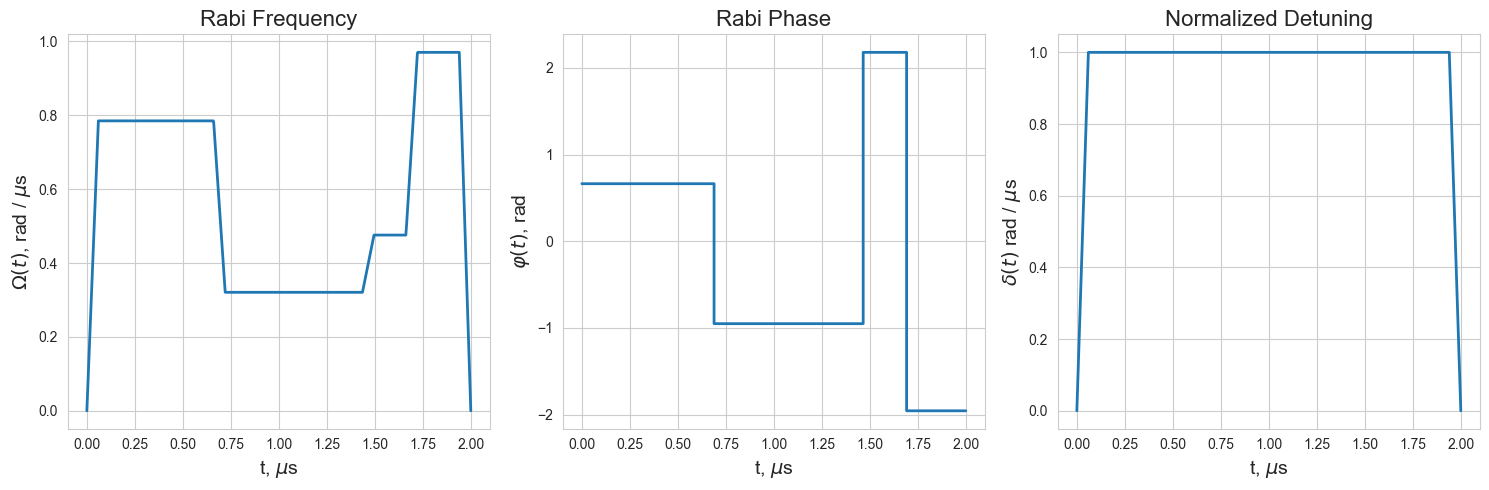
\includegraphics[width=1\linewidth]{figures/parameters_vs_time.png}
    \caption{Пример кусочно-постоянной параметризации временной зависимости $\Omega(t)$, $\varphi(t)$ и $\delta(t)$. Для визуализации выбрано число основных сегментов, равным $4$, при фиксированной длительности линейных переходов $\tau_{\text{trans}} = 0.06 \, \mu s$. Частота Раби $\Omega(t)$ и фаза $\varphi(t)$ имеют одинаковую структуру сегментов. Обучаемыми параметрами являются длительность каждого сегмента, а также значения $\Omega(t)$ и $\varphi(t)$ внутри сегмента. Нормализованный детьюнинг $\delta(t)$ представлен единым сегментом, чья длительность подстраивается под общее время эволюции, определяемое $\Omega(t)$ и $\varphi(t)$. }
    \label{fig:parameters_vs_time}
\end{figure}


\section{Simulation}
\label{seq:simulation}


* Excluding blockaded dimensions: speedup, error vs distance

Для задач квантового машинного обучения разработаны ряд фреймворков \cite{}. Стандартные подходы к оптимизации параметров квантовых систем опираются на эволюцию с использованием параметризованных квантовых гейтов. Такая динамика легко поддаётся симуляции, поскольку сводится к вычислению матричных экспонент от постоянных гамильтонианов. В свою очередь, симуляция эволюции системы ридберговских атомов представляет собой значительно более сложную вычислительную задачу.

Как отмечалось в разделе \ref{seq:qnn intro}, зависимость гамильтонина от времени не позволяет получить оператор эволюции аналитическим способом. В связи с этим, его нахождение требует ресурсоёмких численных методов вычисления Т-экспоненты. Такой подход реализован в библиотеках pennylane и bloqade \cite{}. Следовательно симуляция эволюции даже с одним набором параметров занимает значительное время, что делает непрактичным обучение QML моделей, требующих многократных итераций. Для преодоления этого ограничения нами был разработан симулятор для эффективного расчёта динамики ридберговских систем.

Основынми целями были максимальное ускорение вычислений и реализация параллельной симуляции систем с разными параметрами, что необходимо для batch processing. Поэтому в качестве основного фрейморка был выбран JAX \cite{}, который ускоряет вычисления за счёт JIT-компиляции и предоставляет нативные средства для векторизации операций.



Ключевой проблемой является вычисление Т-экспоненты, решение которой требует упрощения системы. Мы отказались от поддержки произвольных временных зависимостей функций $\Omega(t)$, $\varphi(t)$ и $\delta(t)$, ограничившись их кусочно-постоянной параметризацией, описанной в разделе \ref{seq: qnn intro}. Однако даже при таких условиях эволюция не вычисляется аналитически из-за линейных переходов между сегментами. 

Чтобы свести симуляцию к произведению экспонент от постоянных гамильтонианов, мы аппроксимировали каждый линейный переход равномерно конечным числом кучосно-постоянных шагов. Пример такой аппроксимации представлен на Рисунке \ref{fig:steps_approximation}.  Очевидно, что такой подход вносит контролируемую погрешность в симуляцию, но позволяет кардинально ускорить вычисления, за счёт аналитического рассчёта оператора эволюции. Точность аппроксимации увеличивается с числом шагов, как изображено на Рисунке \ref{fig:errors_comparison} (слева).

\begin{figure}[h!] \label{fig:steps_approximation}
    \centering
    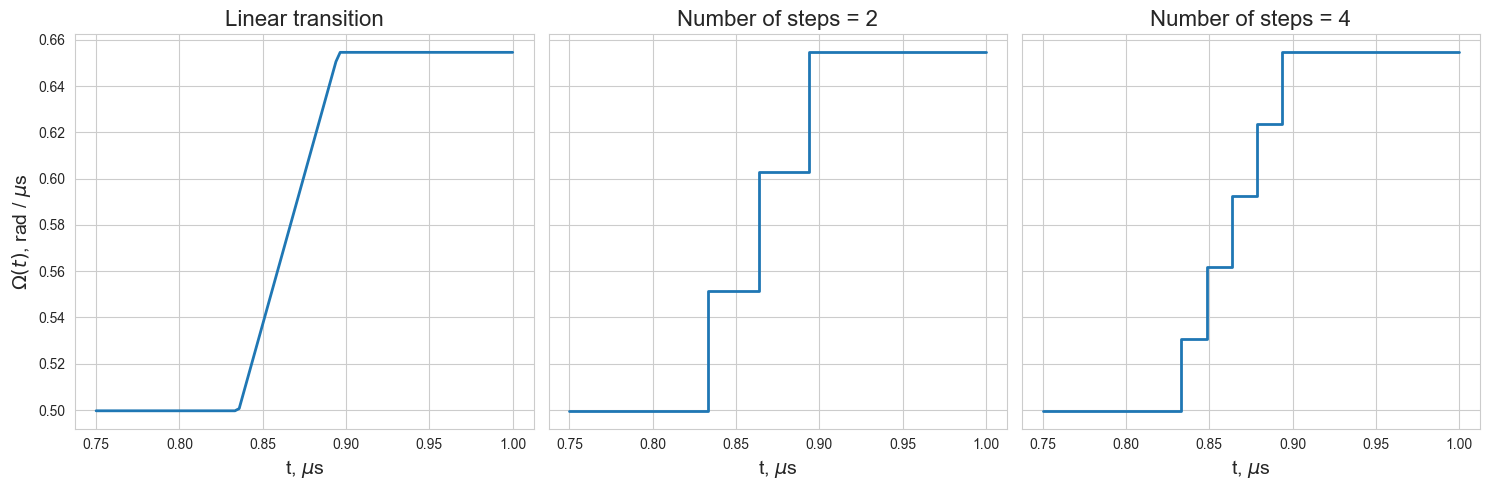
\includegraphics[width=1\linewidth]{figures/steps_plot.png}
    \caption{Пример кусочно-постоянной равномерной аппроксимации одного линейного перехода частоты Раби с использованием двух и четырёх шагов.}
\end{figure}



При работе с реальным квантовым компьютером невозможно измерить конечную волновую функцию. Поэтому средние значения наблюдаемых величин оцениваются посредством многократных проективных измерений, что вносит стастическую ошибку, известную как shot noise. Этот аспект даёт конструктивный физический критерий для выбора числа шагов аппроксимации: нужно увеличивать шаги до тех пор, пока ошибка симуляции не станет сопоставимой с shot noise. Фреймворк bloqade, совместимый с квантовым компьютером Aquila, предоставляет возможность проводить симуляцию его работы с учётом shot noise. На Рисунке \ref{fig:errors_comparison} (справа) представлена зависимость относительная ошибки, вызванной shot noise, от числа шотов. На практике обычно используется $10^3 \sim 10^4$ шотов. Сравнение двух графиков показывает, что использование всего 2 шагов аппроксимации вносит ошибку меньше shot noise в рабочем диапазоне.

\begin{figure}[h!] \label{fig:errors_comparison}
    \centering
    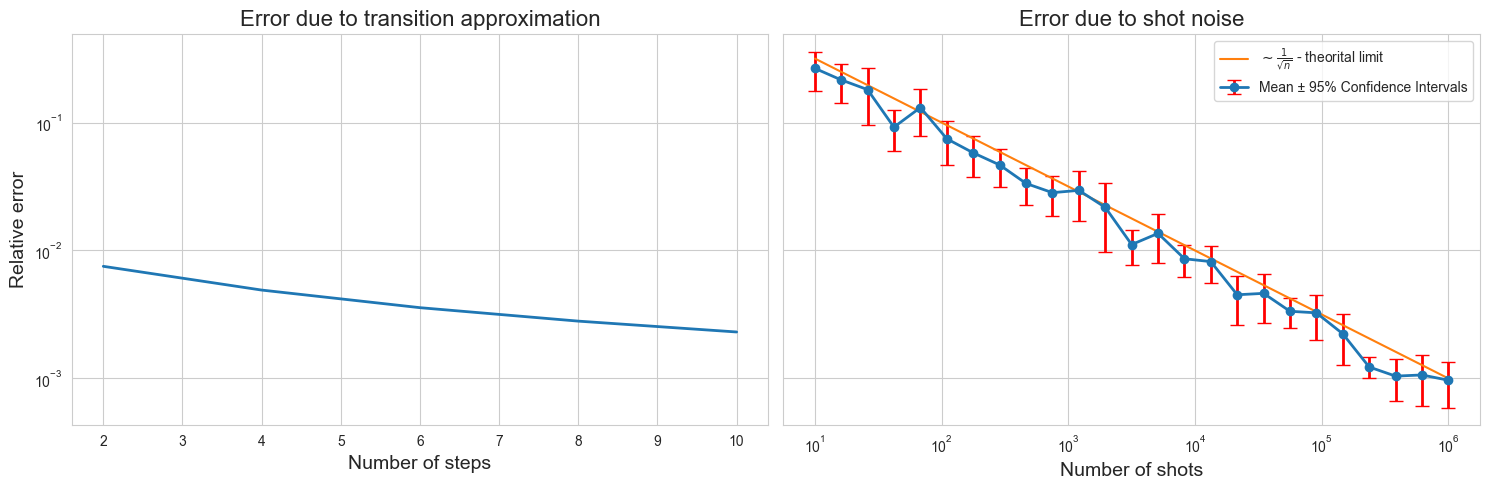
\includegraphics[width=1\linewidth]{figures/errors_plot.png}
    \caption{Сравнение источников ошибки в log-log масштабе. \textbf{Слева:} Зависимость относительной ошибки симуляции от числа шагов аппроксимации. \textbf{Справа:} Зависимость относительной ошибки от числа измерений. Доверительный интервалы построены по результатам 10 экспериментов.  Оранжевая кривая соответствует теоретическому пределу $1 / \sqrt{n}$ , следующему из центральной предельной теоремы \cite{}}
\end{figure}

\subsection{Rydberg Blockade} \label{seq:bloqade}
Одной из ключевых особенностей ридберговских систем является сильное взаимодействие Ван-дер-Ваальса. Как показано в уравнении \ref{eqn:van-der-vaals interaction}, энергия этого взаимодействия $V_{ij} \propto C_6/r_{ij}^6$ убывает с расстоянием $r_{ij}$ и характеризуется аномально большим коэффициентом $C_6$. Поэтому, когда атомы расположены достаточно близко, энергия их взаимодействия может значительно превышать частоту Раби. В этом режиме, известном как \textbf{Ридберговская блокада}, одновременное возбуждение обоих атомов оказывается подавленным.

Эта особенность крайне полезна для симуляции квантовой динамики, поскольку позволяет значительно снизить вычислительные ресурсы. Достигается это с помощью проецирования на эффективное подпространство, из которого исключены запрещённые состояния. Чтобы качественно оценить вклад от этого эффекта, рассмотрим систему из $n$ атомов, расположенных в одномерную цепочку на одинаковом расстоянии друг от друга. Введем параметр <<радиус блокады>> $R_b$, определяющий расстояние, в пределах которого одновременное возбуждение двух атомов запрещено. Будем считать, что этот радиус охватывает $k$ атомов.

Положим $p_n$ ранвым размерности гильбертова пространства разрешённых состояний. В терминах битовых строк $p_n$ равно количеству строк длины $n$, в которых в любом окне длины $k$ содержится не более одной единицы. Легко получить рекурентную формулу для $p_n$, рассмотрев 1-й элемент битовой строки:
\begin{itemize}
    \item Если 1-й элемент равен 0, то он не влияет на ограничения для следующих $n-1$. Значит число таких строк равно $p_{n-1}$.
    \item Если 1-й элемент равен 1, то в силу блокады все следующие за ним $k-1$ биты должны быть нулями. На оставшиеся $n-k$ атомов накладываются исходные ограничения, и число таких конфигураций равно $p_{n-k}$.
\end{itemize}
Суммируя эти два случая, приходим к рекурентному соотношению:
\begin{equation}
    p_n = p_{n-1} + p_{n-k}.
    \label{eqn:blockade_recurrence}
\end{equation}
В качестве граничных условий можно положить $p_n = n+1$ для $1 \le n \le k$, поскольку радиус блокады охватывает всю систему.

Решение данного линейного рекурентного уравнения определяется характеристическими числами, удовлетворяющими уравнению:
\begin{equation}
    x^{k} = x^{k - 1} + 1.
\end{equation}
Оно всегда имеет доминирующий корень $\lambda_k \in (1, 2)$, который определяет асимптотику $p_n \sim c \cdot \lambda_k^n$ \cite{ConcreteMath}. Значит при фиксированном $k$ размерность эффективного гильбертова пространства всё ещё растёт экспоненциально, но с показателем значительно меньшим 2. Зависимость размерности подпространства от параметра $k$ для системы из 10 атомов показана на Рисунке \ref{fig:blockade_analysis} (слева).

\begin{figure}[h!]
    \centering
    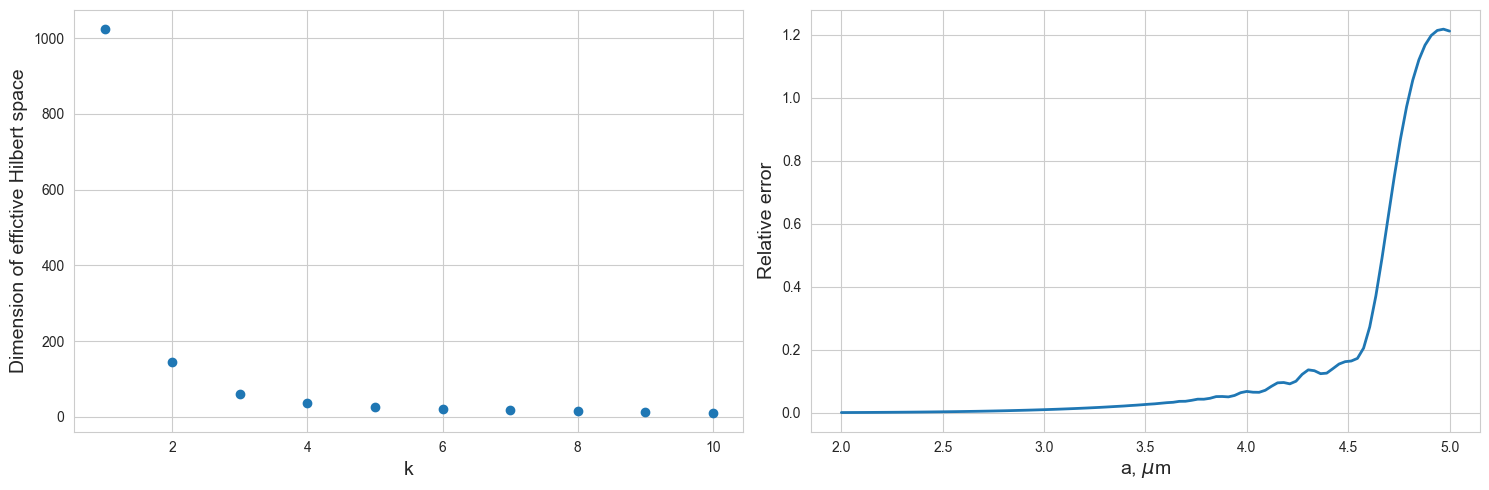
\includegraphics[width=1\linewidth]{figures/bloqade_plot.png}
    \caption{Графический анализ ридберговской блокады. \textbf{Слева:} Зависимость размерности гильбертова пространства разрешённых состояний от числа заблокированных атомов $k$ для цепочки из 10 атомов. Размерность полного пространства $2^{10}=1024$. \textbf{Справа:} Зависимость относительной ошибки аппроксимации ридберговской блокады от расстояния между атомами для системы из 3 атомов. Эффективный радиус блокады $R_b$ соответствует началу экспоненциального роста ошибки и в данном случае равен $4.5 \mu m$.}
    \label{fig:blockade_analysis}
\end{figure}

Остается вопрос об определении радиуса блокады $R_b$, поскольку блокада является аппроксимацией к настоящей эволюции в полном пространстве. Точность этой аппроксимации определяется отношением величины межатомного взаимодейтсвия к параметрам лазерного воздействия. Для численного определения $R_b$ можно использовать следующий подход:
\begin{enumerate}
    \item Радиус блокады полагается условно бесконечным, при котором все атомы заблокированы.
    \item Проводится симуляция с учётом блокады. 
    \item Проводится серия экспериментов с разным расстоянием между атомами без блокады.
    \item Для каждого эксперимента вычисляется ошибка симуляции как относительная норма разности конечных волновых функций.
\end{enumerate}
На графике зависимости ошибки симуляции от расстояния $a$ будет наблюдаться следующее поведение: при малых $a$ ошибка мала, но по мере увеличения расстояния начинается экспоненциальный рост. Точка, соответствующая переходному моменту принимается за эффективный радиус блокады $R_b$. Пример такого графика показан на Рисунке \ref{fig:blockade_analysis} (справа).

\section{Results}
\subsection{Постановка основных экспериментов}
В качестве основной модели для проведения численных экспериментов выбрана архитектура из $N = 4$ ридберговских атомов, расположенных в узлах квадратной решётки. Временная зависимость параметров гаильтониана, описанная в пункте \ref{seq:simulation}, разбивалась на $\text{num\_time\_segments} = 5$ сегментов. Данная конфигурация является приемлемым компромиссом между выразительностью модели и вычислительными затратами на симуляцию её динамики.

На выходе квантовой сети производилось измерение одно- и двухкубитных наблюдаемых Паули ($Z_i$ и $Z_i Z_j$). Полученные значения подавались на обучаемый линейный слой для отображения в пространство признаков, соответствующее числу классов решаемой задачи. В такой постановке для задачи бинарной классификации общее число обучаемых параметров модели составило $103$.

\begin{figure}[h!]
    \centering
    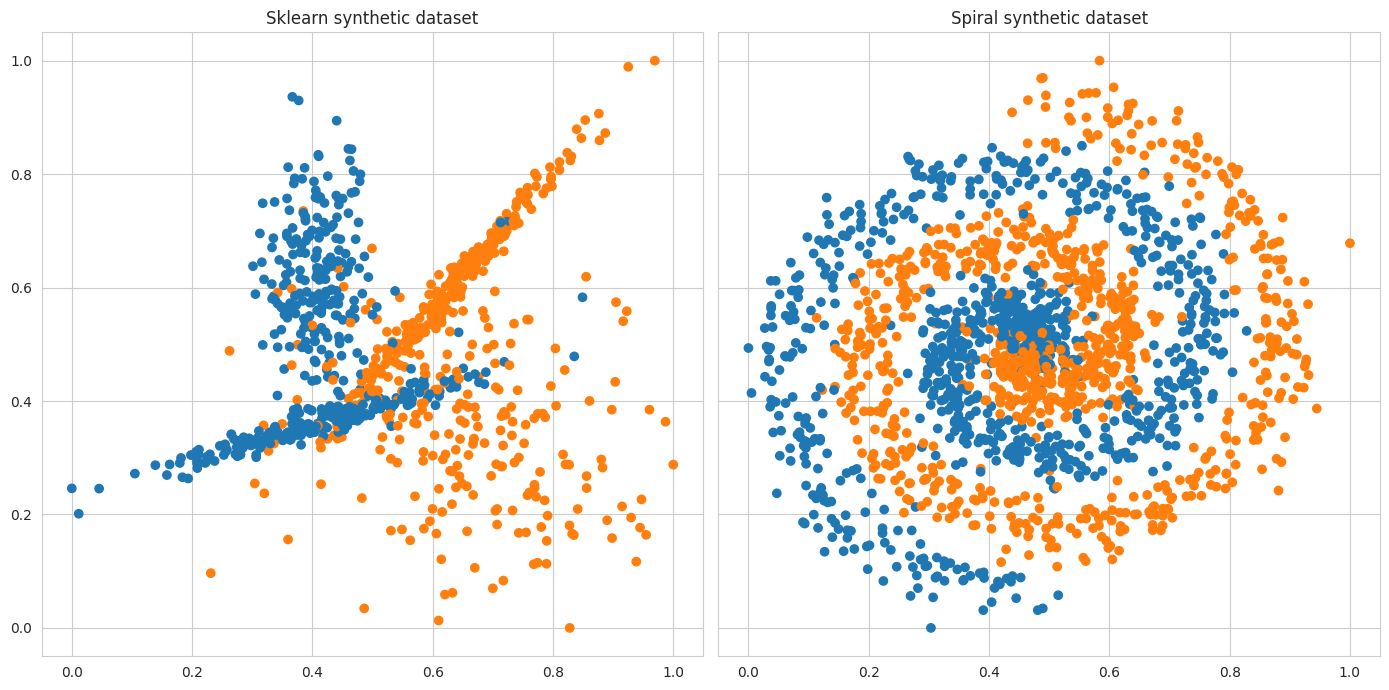
\includegraphics[width=1\linewidth]{figures/datasets.png}
    \caption{Синтетические датасеты для обучения. \textbf{Слева:} многомерная классификация (сгенерирована функцией \texttt{make\_classification}). На графике приведен двумерный вариант для визуализации; в основных экспериментах использовалось 4 признака. \textbf{Справа:} Зашумлённый спиральный датасет, который служит для проверки экспрессивности квантовой модели.}
    \label{fig:datasets}
\end{figure}

В предлагаемом подходе входные признаки распределяются по схеме «один признак на один атом». Учитывая высокую вычислительную сложность рассчёта прямого и обратного подхода по квантовой сети, для обучения были выбраны два компактных синтетических набора данных. Все входные значения были отнормированы в диапазон $[0, 1]$. Визуализация тренировочных данных представлена на Рисунке \ref{fig:datasets}.

Выбор и конфигурация датасетов обусловлены необходимостью строгого разделения классического и квантового вклада в итоговый результат:
\begin{enumerate}
    \item \textbf{Многомерная классификация (4 признака):} сгенерирован с помощью функции \texttt{make\_classification} (библиотека scikit-learn). Использовалась конфигурация с 4 признаками и 2 кластерами на класс. Это позволило реализовать прямую передачу данных в квантовый слой без использования промежуточного классического линейного слоя, изменяющего размерность. Такой подход является методологически важным: поскольку задача потенциально допускает достижение приемлемой точности даже линейными методами, исключение обучаемого препроцессинга позволяет изолированно измерить влияние квантовой архитектуры на качество классификации.
    \item \textbf{Спиральный датасет (2 признака):} сгенерирован для оценки экспрессивности предложенной архитектуры при решении существенно нелинейных задач. В этой постановке использовался минимальный линейный слой для отображения двух входных признаков на четыре атома системы. Важно отметить, что в силу топологии <<спирали>>, линейное преобразование само по себе не способно упростить задачу классификации. Таким образом, высокая точность, достигнутая на данном датасете, может быть интерпретирована как доказательство нетривиальности работы квантового слоя.
\end{enumerate}

Подбор гиперпараметров (начальные длительности импульсов, амплитуды, межатомное расстояние и скорость обучения) осуществлялся с использованием байесовской оптимизации (библиотека Optuna). Для каждого набора данных было проведено 400 итераций поиска (trials) длительностью по 500 эпох каждая. Пределы learning\_rate были выставлены так, что за такое число эпох любой запуск сходился.

В качестве бейзлайна была выбрана архитектура MLP с одним скрытым слоем. Размер скрытого слоя подбирался таким образом, чтобы число тренируемых параметров MLP совпадало с квантовой архитектурой.

\subsection{Анализ графиков обучения}

На Рисунке \ref{fig:training_curves} представлены результаты обучения разных конфигураций модели на двух датасетах. Сравнительный анализ графиков позволяет сделать следующие выводы:
\begin{itemize}
    \item \textbf{Экспрессивность.} На спиральном наборе данных (Рисунок \ref{fig:results_spiral}) наблюдается ярко выраженное преимущество: в то время как классический MLP-бейзлайн с эквивалентным числом параметров демонстрирует не способность решить задачу, квантовая модель достигает практически идеальной классификации.
    \item \textbf{Роль квантовой запутанности.}Абляционное исследование выявило критическую важность взаимодействия между атомами. В режиме «disentangled» (искусственное выключение взаимодействия в гамильтониане) и при исключении двухкубитных корреляторов из измерений наблюдается заметная деградация модели. Это доказывает, что квантовая запутанность вносит существенный вклад в работоспособность предложенной архитектуры.
    \item \textbf{Численная устойчивость.} Для всех конфигураций модели на основе ридберговских атомов характерны сильные флуктуации кривых обучения. Это обусловлено высокой чувствительностью функции потерь к параметрам лазерных импульсов в окрестности ридберговской блокады. Несмотря на это, повторяющаяся тенденция к уменьшению тренировочного лосса подтверждает робастность обучения предложенной архитектуры.
\end{itemize}

\subsection{Анализ гиперпараметров}

\begin{figure}[h!]
    \centering
    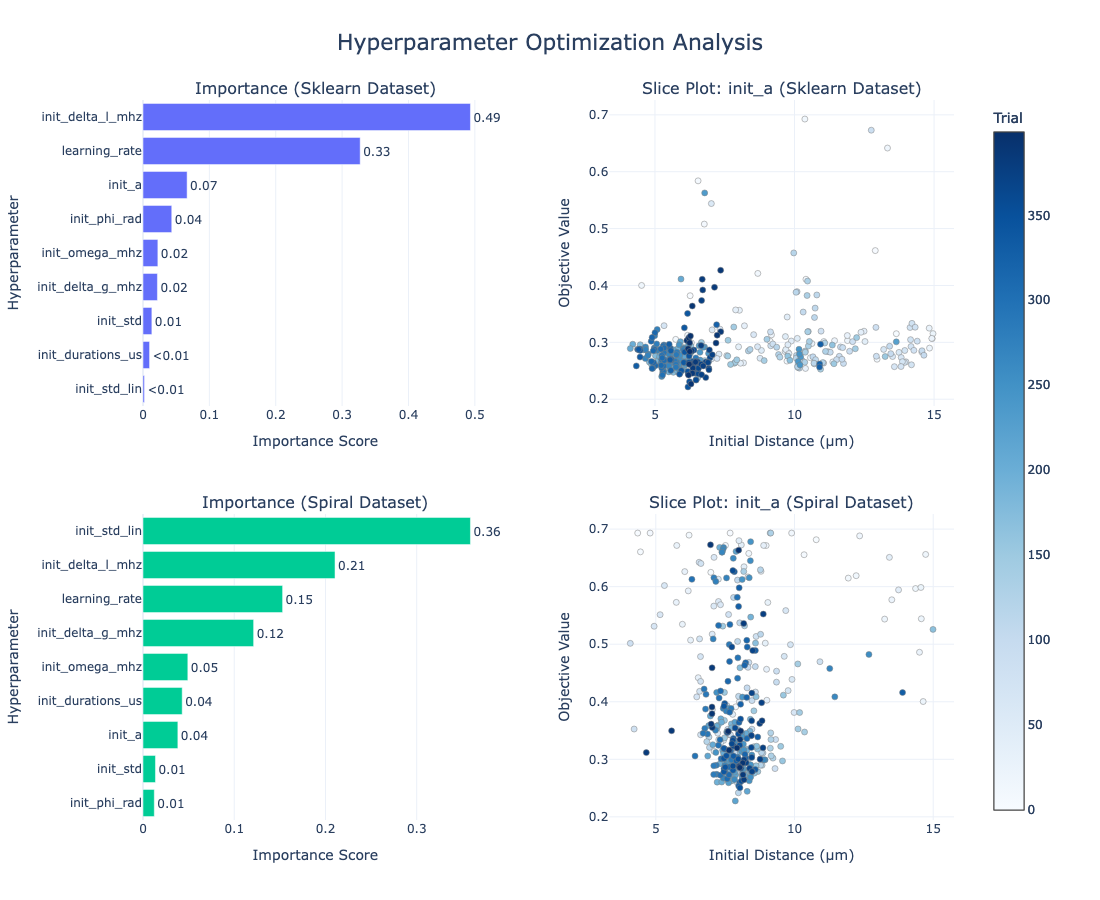
\includegraphics[width=0.8\linewidth]{figures/hyperparam_optimisation.png}
    \caption{Сравнительный анализ оптимизации гиперпараметров для многомерного (верхний ряд) и спирального (нижний ряд) датасетов.}
    \label{fig:hyperparams}
\end{figure}

Для интерпретации механизмов обучения предложенной архитектуры был проведен анализ результатов оптимизации гиперпараметров (Рисунок \ref{fig:hyperparam_optimisation}). Полученные данные позволяют выделить ключевые факторы, определяющие производительность квантовой нейронной сети на основе ридберговских атомов.

\begin{itemize}
    \item \textbf{Роль детьюнинга и кодирования признаков.} Согласно графикам важности признаков (Hyperparameter Importance), критическую роль во всех экспериментах играет начальный масштаб локального детьюнинга (\texttt{init\_delta\_l\_mhz}), а в случае спирального датасета — также инициализация весов классического линейного слоя (\texttt{init\_std\_lin}). Физическая интерпретация данного результата легко объясняется способом кодирования входящих данных в гамильтониан. Из формулы \ref{eqn:detuning parametrisation} следует, что только локальный детьюнинг определяет итоговый вклад изначальных фичей в квантовую эволюцию. Высокая важность этого параметра указывает на то, что для эффективного обучения квантовой сети необходимо правильно подбирать масштаб членов в гамильтониане. В случае спирального датасета используется линейный препроцессинг перед подачей данных в квантовый слой, который выполняет аналогичную масштабирующую функцию, что подтверждается весомым вкладом гиперпараметра \texttt{init\_std\_lin}.
    \item \textbf{Влияние начального межатомного расстояния}. Анализ Slice Plot по параметру начального расстояния между атомами (\texttt{init\_a}) позволяет сделать выводы о чувствительности модели к взаимодействию между атомами. Несмотря на то, что одномерное сечение не способно полностью отразить многомерный ландшафт функции потерь, на графиках отчётливо заметна область оптимальных значений данного гиперпараметра. В обоих случаях данная область находится в диапазоне $5$--$10$~мкм. Такие расстояния достаточно велики, чтобы не реализовывалась ридберговская блокада, но малы, чтобы полностью не учитывать взаимодействие. Это служит косвенным подтверждением реализации <<квантового преимущества>>: успешное решение классической задачи происходит за счёт многочастичных корреляций.
    \item \textbf{Потенциал упрощения обучения}. Интересным наблюдением является минорный вклад остальных <<физических>> гиперпараметров, таких как начальные частота Раби (\texttt{init\_omega\_mhz}), фаза (\texttt{init\_phi\_rad}) и длительность эволюции (\texttt{init\_durations\_us}). Данный факт позволяет в практических реализациях зафиксировать эти параметры стандартными значениями без существенной потери выразительной способности сети и тем самым сократить пространство поиска гиперпараметров.
\end{itemize}


\begin{figure}[p] % [p] вынесет графики на отдельную страницу, если они крупные
     \centering
     \begin{subfigure}[b]{0.8\textwidth}
         \centering
         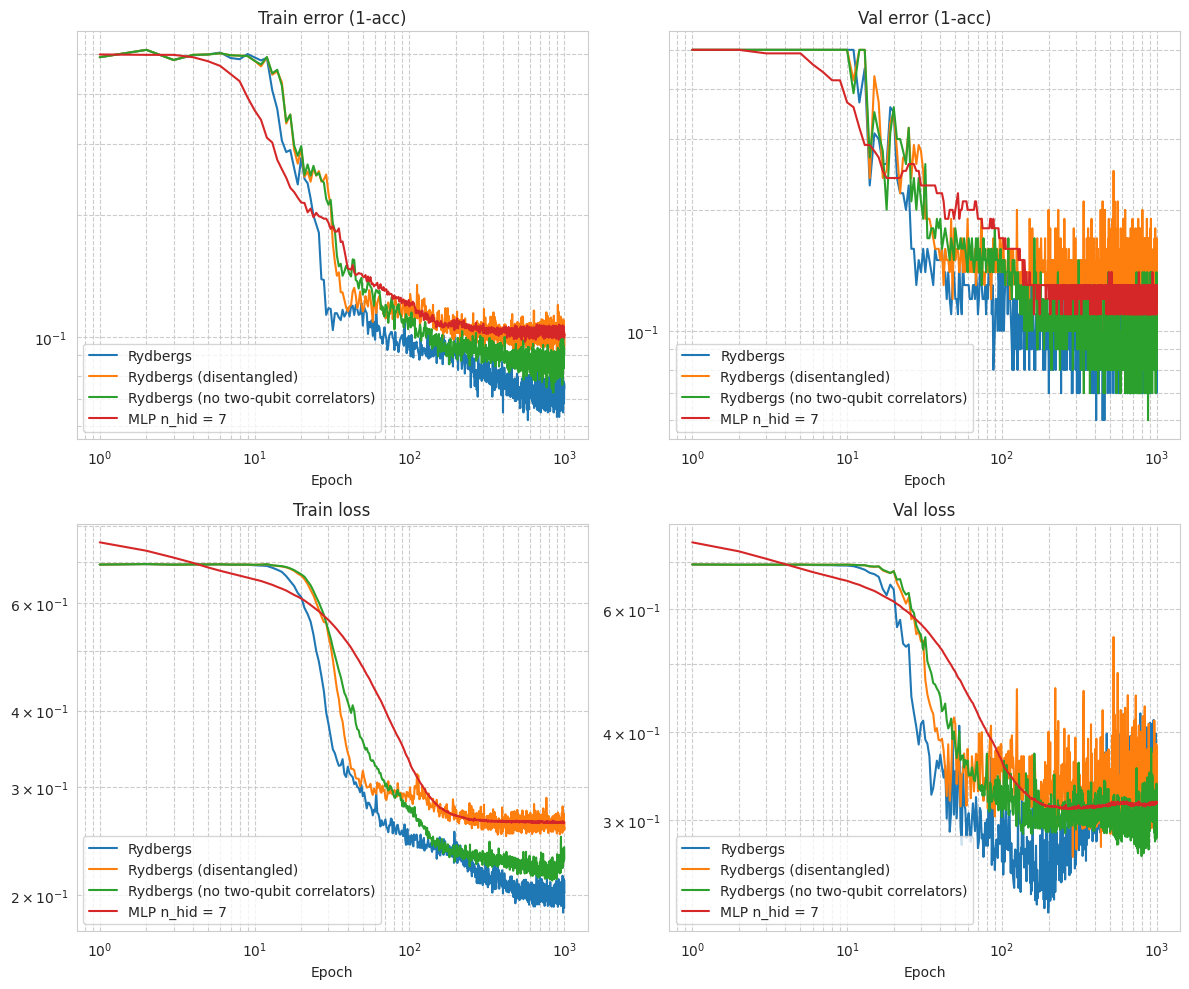
\includegraphics[width=\linewidth]{figures/sklearn_results.png}
         \caption{Многомерный датасет (4 признака).}
         \label{fig:results_sklearn}
     \end{subfigure}
     \vspace{0.5cm} % Отступ между верхним и нижним графиком
     \begin{subfigure}[b]{0.8\textwidth}
         \centering
         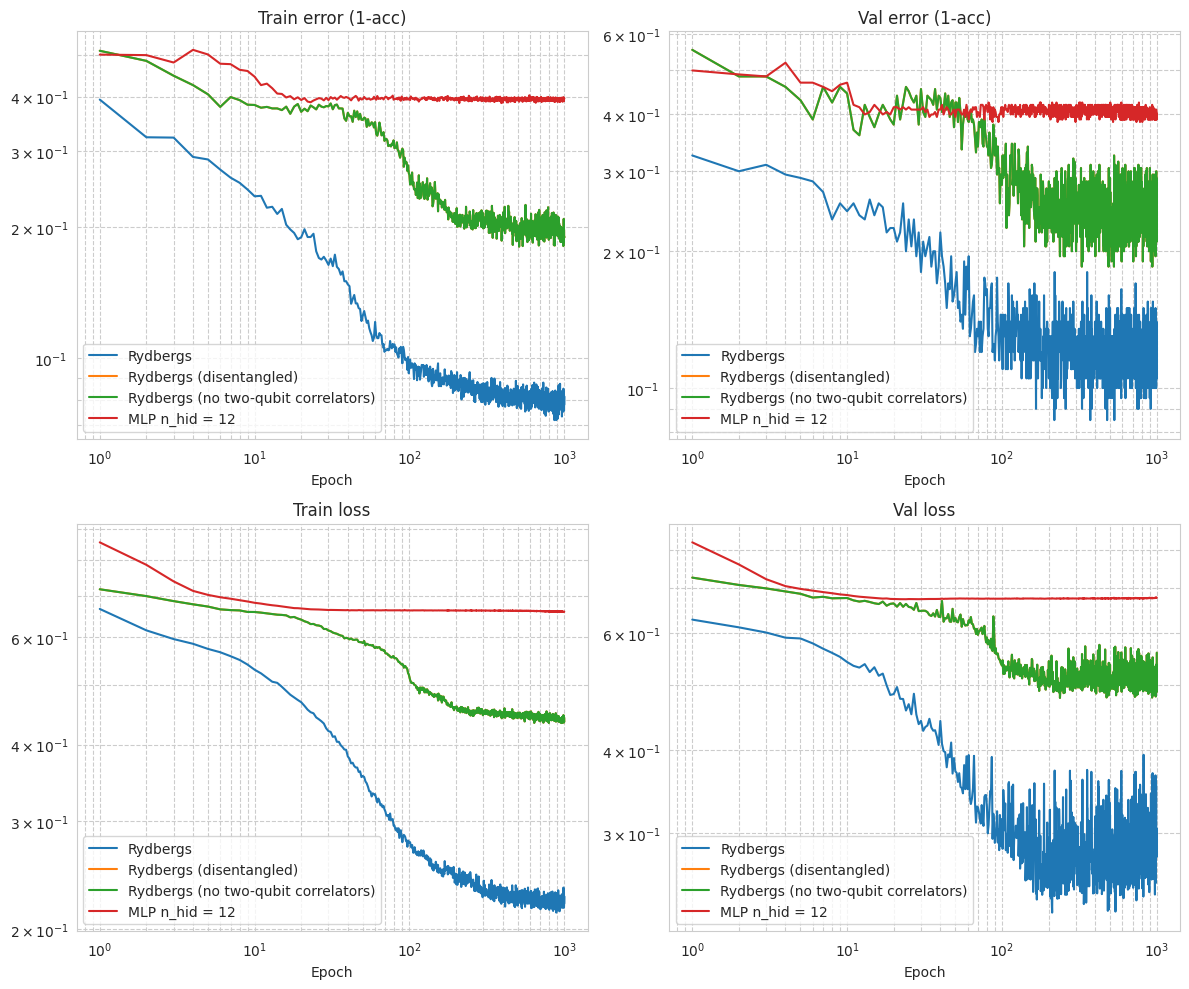
\includegraphics[width=\linewidth]{figures/spiral_results.png}
         \caption{Спиральный датасет (2 признака).}
         \label{fig:results_spiral}
     \end{subfigure}
     \caption{Кривые обучения (Train/Val Error и Loss) для предложенной архитектуры на базе ридберговских атомов и классического MLP-бейзлайна. Сравнение включает полную модель, режим без межатомного взаимодействия (disentangled) и вариант без использования двухкубитных наблюдаемых.}
     \label{fig:training_curves}
\end{figure}


\newpage
\bibliography{lib}
\bibliographystyle{unsrt}


\end{document}
